%====================================================
%  Dark Energy / Late-Time Cosmology Template
%====================================================

\documentclass[
    aps,
    prd,
    twocolumn,
    nofootinbib,
    floatfix,
    superscriptaddress
]{revtex4-2}

%----------------------------------------------------
% Encoding & Fonts
%----------------------------------------------------
\usepackage[T1]{fontenc}
\usepackage[utf8]{inputenc}
\usepackage{lmodern}

%----------------------------------------------------
% Mathematics
%----------------------------------------------------
\usepackage{amsmath, amssymb, amsfonts}
\usepackage{mathtools}
\usepackage{physics}
\usepackage{bm}

%----------------------------------------------------
% Figures & Tables
%----------------------------------------------------
\usepackage{graphicx}
\usepackage{booktabs}
\usepackage{array}

%----------------------------------------------------
% Typography
%----------------------------------------------------
\usepackage{microtype}
\usepackage{enumitem}
\setlist{nosep}

%----------------------------------------------------
% Hyperlinks
%----------------------------------------------------
\usepackage[
    colorlinks=true,
    linkcolor=blue,
    citecolor=blue,
    urlcolor=blue
]{hyperref}

%----------------------------------------------------
% Dark Energy & Cosmology Macros
%----------------------------------------------------

% Omegas
\newcommand{\Om}{\Omega_{\mathrm{m}}}
\newcommand{\Ol}{\Omega_\Lambda}

% Energies
\newcommand{\Ep}{E_\mathrm{peak}}
\newcommand{\Ei}{E_\mathrm{iso}}

%----------------------------------------------------
% Title Information
%----------------------------------------------------
\begin{document}
\title{Cosmological Parameter Inference with Amati GRB relation}

\author{Joan Alcaide-Núñez}
\affiliation{Osservatorio Astronomico di Brera (OAB-INAF), Merate, Italy}

\date{\today}

\maketitle

%----------------------------------------------------
% Abstract
%----------------------------------------------------
\begin{abstract}
Should I include the SGRB fits when the results are ready? Should I include the results from the $\chi^2$-volume for H0OmOL?
\end{abstract}

%----------------------------------------------------
% Document
%----------------------------------------------------

% \tableofcontents
\vspace{1em}

%====================================================
\textit{This document summarizes an independent research project under the scientific guidance of Dr. Giancarlo Ghirlanda and Dr. Om Sharan Salafia. The work is exploratory in the nature and intended as a research report for training purposes and is not a peer-review publication.
}

%====================================================
\section{Introduction}
%====================================================

The accelerated expansion of the Universe remains one of the central open problems in modern cosmology. Whiel the standard $\Lambda$CDM model has provided an excellent phenomenological description of a range of observations, the physical nature of dark energy and the precise values of cosmological parameters continue to be actively discussed. In recent years, increasing attention has been drawn to the so-called Hubble tension, the persistent discrepancy of measurements of the Hubble constant ($H_0$) inferred from early-Universe probes and the late-time distance ladder. This tension has motivated the expliration of complementary and independent cosmological probes.

Gamma-ray bursts (GRBs) are among the most luminous transient phenomena in the Universe and are detectable over a broad redshift range, extending well beyond that of Type Ia supernovae and any other standard candle. Their luminisities make them appealing candidates for cosmological sutides, particularly at high redshift. However, unlike supernovae, GRBs are nto standard candles. Their use as distance indicators relies on empirical correlations between observable properties. %such as the relation between the rest-frame spectral peak energy $\Ep$ and the isotropic equivalent energy $\Ei$.
While such correlations have been extensively studied, their physical origin, intrinsic scatter, and susceptibility to selection effects remain subjects of ongoing debate.

In parallel, gravitational-wave (GW) observations have openened a new avenue for cosmology. Compact binary mergers with electromagnetic counterparts provide direct measurements of luminosity distance indepent of the cosmic distance ladder, earning the designation of "standard sirens". Although the current number of observed multi-messenger events is limited to one \cite{PhysRevLett.119.161101}, coming observations campaigns \cite{Salafia_2025} and future GW detectors, such as Einstein Telescope or Cosmic Explorer, are expected to increase the available sample, making standard sirens a promising tool for precision cosmology.

The aim of this project is to explore, within a simplified framework, the use of GRB empirical relations as cosmological probes and examine potential of GW detections for the same purpose. The focus lies on feasibility, identifying dominant limitations and illustrating the complementarity of EM and GW observations.

To this end, $(\Om, \Ol)$ cosmological parameter space are inferred by fitting the $\Ep-\Ei$ phenomenological relation across using a $\chi^2$ minimization approach. Independent constraints are then also drawn from simulated binary neutron star mergers, finally combining both probes to visualize a basic multi-messenger inference process. This report is structured as follows: Section \ref{sec:methodology} defines the cosmological framework and the fitting process for both the GRB relation and GW Hubble diagram. Section \ref{sec:data} describes the used datasets to obtain the results presented in section \ref{sec:results}. In section \ref{sec:discussion}, I discuss the limitations and room for improvement of this basic analysis, which leads to outlining directions for future improvemets in section \ref{sec:future}.

%====================================================
\section{Methodology}\label{sec:methodology}
%====================================================

\subsection{Cosmological Framework}

Throughout this work, I assume a flat $\Lambda$CDM cosmological model, characterised by the matter density parameter $\Om$ and the dark energy density parameter $\Ol$ (with $\Omega_k = 0$). The contribution of radiation is neglected ($\Omega_r = 0$), as it is subdominant over the redshift range relevant to the present analysis. The Hubble constant is fixed to $H_0 = 70.0\ \mathrm{km s^{-1} Mpc^{-1}}$ allowing for the exploration of the $(\Om, \Omega_\Lambda)$ parameter space without introducing additional degeneracies. Under this assumptions the luminosity distance is given by:
\begin{equation}
    d_L (z) = (1+z)\frac{c}{H_0} \int_0 ^z \frac{dz^\prime}{\sqrt{\Om(1+z^\prime)^3+\Omega_\Lambda}}
\end{equation}

which is evaluated numerically using standard routines from the \verb|astropy.cosmology| library.

\subsection{GRB Empirical Relation}

The analysis is based on the empirical correlation between the rest-frame peak energy $\Ep$ and the isotropic equivalent energy $\Ei$, commonly referred to as the Amati relation \cite{ghirlanda_2006}. In logarithmic form, this relation can be written as
\begin{equation}
    \log_{10} \Ep = a \log_{10} \Ei + b
\end{equation}
where $a$ and $b$ are free parameters describing the slope and normalisation of the correlation respectively. The isotropic energy depends explicitly on the assumed cosmology through the luminosity distance,
\begin{equation}
    \Ei = 4\pi d_L(z) \mathcal{F}/(1+z)
\end{equation}
where $\mathcal{F}$ is the observed fluence and $z$ the source redshift.

Due to this dependecy, the parameters of the $\Ep-\Ei$ relation, and its goodness of fit, vary across the cosmological parameter space $(\Om, \Omega_\Lambda)$. In this work, the physical origin of the empirical correlation is nto modeled, treating the relation phenomenologically, with the goal of assessing its utility as a cosmological probe under simplified assumptions.

\subsection{Parameter Estimation via $\chi^2$ Minimization}

As mentioned above, GRB are not standard candles like Ia supernovae, since the $\Ep-\Ei$ relation parameters are different with varying cosmologies. The circularity problem is that in order to know $\Ep$ and fit the correlation we need to assume a cosmology, since $\Ep$ depends on $d_L$. One of the solutions to this issue in the literature is to fit the GRB correlation for all possible cosmoslogies (within some logical limits) and building a $\chi^2(\Om, \Ol)$ surface. Then, the cosmology with minimum $\chi^2$ is expected to be the 'best' cosmology.

For a given choice of $(\Om, \Ol)$, the GRB correlation parameters $a$ and $b$ are determined by minizing a $\chi^2$ statistic defined as

\begin{equation}
    \chi^2 = \sum_i \frac{\left[\log_{10}\Ep_{,i}-(a\log_{10}\Ei_{,i}+b)\right]^2}{\sigma_{\log \Ep_{,i}} ^2 + \sigma_\mathrm{extra} ^2}
\end{equation}

where $\sigma_{\log \Ep_{,i}}$ denotes the measurement uncertainty of $\log_{10} \Ep$ and $\sigma_\mathrm{extra}$ is a correlation intrinsic scatter term introduced to account for scatter larger than the measurement uncertainty itself. During the analysis this was set to $\sigma_\mathrm{extra} = \log_{10} (1.3) \approx 0.114$ and held fixed throughout cosmologies. By minimizing the $\chi^2$ fit of the parameters we obtain the $\Ep-\Ei$ relation and the $chi^2$ surface point for that cosmology. The location of the minimum and the $chi^2$ contours provide an estimate of the 'best' cosmological parameters.

%Considering the adopted framework, simplified assumptions and fitting resolution, these constraints are interpreted as indicative rather than measurements. % move to results

\subsection{Gravitational Wave Standard Sirens}

In addition to GRB-based constraints, gravitational-wave standard sirens can be used to provide an independent probe of cosmology. The strain of a gravitational-wave provides information about the (luminosity) distance of the source, with a certain amount of degeneracy with the system plane angle. When a gravitational wave signal is associated with an electromagnetic counterpart, the redshift of the source can be measured directly, allowing the luminosity-distance-redshift relation (Hubble diagram) to be constrained without reliance on the cosmic distance ladder.

Due to the limited number of observed multi-messenger events to date, a simulated population of binary neutron star mergers (BNS) is employed. The simulated dataset provides redshift and luminosity distance measurements, which are fitted using the same luminosity distance expression as above. Cosmological constraints are inferred by minimizing the reduced $\chi^2$ with the constructed Hubble diagram:

\begin{equation}
    \chi^2 = \frac{1}{\mathcal{N}} \sum_i \frac{\left[d_L(data) - d_L(z, \Om, \Ol)\right]^2}{\sigma_{d_L} ^2}
\end{equation}

where $\mathcal{N} = N - 2$ are the degrees of freedom, computed from the number of data points $N$ and the number of fitting parameters $2$.

The use of simulated data allows for a controlled assessment of the constraining power of standard siren, but does not capture all source of observational uncertainty expected in real detections. % CHECK: is this sentence correct?

\subsection{Combined Constraints}

Finally, the GRB-based and GW-based $\chi^2$ surfaces are combined by summing them, assuming statistical independence between the two probes. The resulting joint $\chi^2$ ilusstrates the complementarity of electromagnetic and GW observations in constraining cosmological parameters. The combined results are intendede as a proof of concept rather than a statistically rigorous joint analysis (be reminded that simulated data is in use), highlighting the potential for multi-messenger approaches under simplified assumptions. This methodology does not include effects such as selection biases, redshift evolution of the GRB correlation, correlated uncertainties, and full Bayesian inference, which are deferred to future work.

%====================================================
\section{Data and Assumptions}\label{sec:data}
%====================================================

The data for the GRB observations I extracted from \cite{ghirlanda2008peak}, which representa a table of observed GRB properties from different sources. I used the \verb|Epeak|, \verb|Epeak_err|,\verb|Eiso|,  and \verb|z| columns. The redshift range of the samples is $0.125<z<4.9$. From the original table 2 sources were excluded from this analysis due to their exceptionally low $\Ep$, on order of magnitude smaller.

When employing this dataset, I assume that potential effects such as redshift evolution or selection biases where negligible and that the authors originally computed the $\Ep$ with the same assumptions as here and with the standard values $\OL = 0.7 = 1-\Om$.

For the GW data we used the simulation results by \cite{colombo2025multi}, who simulate $10^4$ binary neutron star merger events including the appearance of kilonovae and GRBs and their properties. From this dataset I only take the luminosity redshift and luminosity distance of the GW events. While the construction of the standard siren Hubble diagram, the issue appeared that I was unable to fit the parameter with $10^4$ data points. Hence the sample is reduced to the first $1000$ in the dataset.

The redshift range is approximately up to $z\sim2$. I assume that this dataset also does not introduce any effects such as redshift evolution or selection biases. However, the cosmological parameters are directly fitted and thus the assumption that the original data follows the standard cosmology is not necessary. Additionally, the luminosity distance uncertainty was set to $\sigma_{d_L} = 0.1 d_L$ for every data point.

%====================================================
\section{Results}\label{sec:results}
%====================================================

\subsection{Constraints from GRB Relations}

Using the methodology described before, the correlation was fitted across a grid in the $(\Om, \Ol)$ parameter space. For each cosmology the $\Ep-\Ei$ correlation was fitted through $\chi^"$ minimization, which was recorded as the cosmology's goodness of fit. This forms a $\chi^2(\Om, \Ol)$ surface which identifies a preferred region in the parameter space, with a minimum ocurring at 
\begin{equation}
    \Om = 0.121 \mathrm{\ and\ } \Ol = 0.970.
\end{equation}

corresponding to a total $\chi^2$ value of $74.95$. Fig. \ref{fig:grb} illustrates this surface showing the confidence contours at the $68\%, 90\%$ and $99\%$ levels. The contours are broad and elongated, reflecting the intrinsic scatter, large uncertainties and the degeneracy of both parameters.

\begin{figure}
    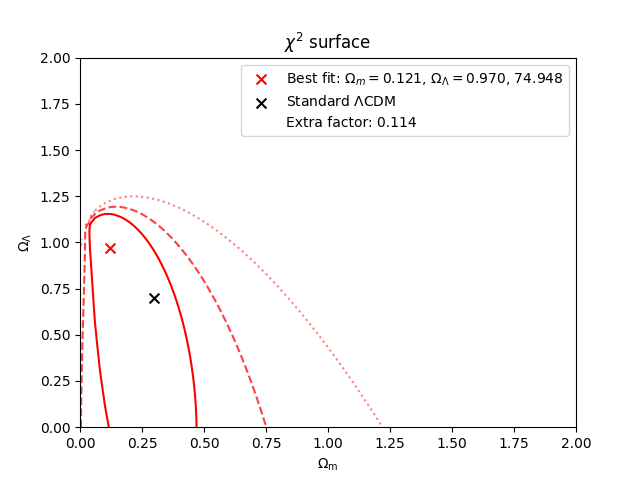
\includegraphics[width=0.9\columnwidth]{GRB_surface.png}
    \caption{$\chi^2(\Om, \Ol)$ surface from GRB Amati relation fits. Confidence contours are shown at $68\%$, $90\%$, and $99\%$ levels, with the best-fit at $\Om = 0.121$ and $\Ol = 0.970$.}
    \label{fig:grb}
\end{figure}

WIthin uncertainties, the inferred parameter rages are broadly consistent with a flat $\Lambda$CDM cosmology. Moreover, the statistical strength is significantly weaker than compared to those obtained from established probes such as Type Ia supernovae or CMB measurements. This highlights the pre-matureness of the and current limitations of the GRB-based cosmological inference. 

\subsection{Constraints from GW Standard Sirens}
A Hubble diagram was constructed using the luminosity distance and redshift of the simulated sample, which was fitted within the same cosmological framework applying a $\chi^2$ statistic as already described. This yields best-fit parameters
\begin{equation}
    \Om = 0.000 \mathrm{\ and\ } \Ol = 0.000.
\end{equation}

The corresponding confidence contours are shown in Fig. \ref{fig:gw}. Compared to the GRB-based constraints, these exhibit a different degeneracy direction in the parameter plane, reflecting the unrelated physical origin of the measurements.

\begin{figure}
    \includegraphics[]{}
    \caption{}
    \label{fig:gw}
\end{figure}

Although this is a simulation and does not capture all the observational uncertainties and effects, the results illustrate the potential of standard sirens as an independent cosmological probe. This is especially compelling in the context of next-generation detectors.

\subsection{Combined GRB \& GW Constraints}

To explore the complementarity of GRB and GW observations, the $\chi^2$ derived from each analysis is finally combined by summation, assuming statistical independence between the two surfaces. The resulting $\chi^2$ joint surface yields a best-fit at 
\begin{equation}
    \Om = 0.000 \mathrm{\ and\ } \Ol = 0.000.
\end{equation}

with a minimum value of $\chi^2 = 00.00$. The correspoding confidence contours are shown in Fig. \ref{fig:joint}, which displays tighter constraints than those obtained from either probe alone. The region of uncertainty lies close to the standard cosmological values. These results are to be viewed as a proof of concept illustrating how multi-messenger observations and cosmological fits can reduce parameter uncertainties.

%====================================================
\section{Limitations and Discussion}\label{discussion}
%====================================================

These results should be interpreted as a proof of concept demonstrating how multi-messenger observations can reduce parameter degeneracies. Given the simplified assumptions and the use of simulated data, the combined constraints are not intended as statistically rigorous measurements.

What limits the analysis
What dominates uncertainty
What could bias results
Why this is not yet publication-ready

single most important section together with methodology

%====================================================
\section{Future Work}\label{sec:future}
%====================================================

Bayesian inference upgrade
Selection effects modeling
GW standard sirens integration
Next steps in realism

One paragraph summarising, emphasising learning outcomes and "This project provided early experience with cosmological inference using non-standard probes and highlighted both the potential and limitations of GRB-based approaches."

%----------------------------------------------------
% Acknowledgments
%----------------------------------------------------
\begin{acknowledgments}
I would like to thank Dr. Giancarlo Ghirlanda and Dr. Om Sharan Salafia for their guidance to this project. I would also like to thank Dr. Gabrielle Ghisellini, Stella Boula and Dr. Lara Nava for insightful discussion. This project was possible thanks to the \textit{Youth and Science} program by \textit{Fundació Catalunya La Pedrera}. % alguien mas en las discussions?
\end{acknowledgments}

%----------------------------------------------------
% Bibliography
%----------------------------------------------------
\bibliographystyle{apsrev4-2}
\bibliography{references}

\end{document}
